\documentclass{article}
\usepackage{fullpage,amsmath,amsthm,graphicx,enumitem}
\usepackage{tikz}
\usepackage{multicol}

\theoremstyle{definition}
\newtheorem{thm}{Theorem}
\newtheorem{question}[thm]{Question}
\newenvironment{solution}{\noindent\textit{Solution:}}{}

\title{ASEN 6519-007 Decision Making under Uncertainty\\
       Homework 1: Probabilistic Models}

\begin{document}

\maketitle

\section{Conceptual Questions}

\begin{question}
There is a 1\% chance there is both life and liquid water on Mars, a 1\% chance there is life but no
water, and a 4\% chance there is no life and no water. What is the probability that there is life on Mars given that there is water?\footnote{These probabilities are totally made up. If you have strong feelings about the real probability of life on Mars, feel free to speculate in your answer :)}
\end{question}

\begin{question}
    Suppose that a stochastic process $\{x_t\}$ is defined by the following equation: $x_{t+1} = x_t + x_{t-1} + v_{t}$ where $v_t$ are i.i.d. noise random variables. Is this process Markov if the state is defined as $x_t$? What would need to be included in the state at time $t$ to make this a Markov process?
\end{question}

\begin{question}
Suppose your company has a dataset with the following variables:
\begin{itemize}[noitemsep]
    \item $S$: a binary variable indicating whether it has snowed in the last two days.
    \item $T$: a binary variable indicating whether the temperature is above or below freezing.
    \item $D$: a binary variable indicating whether the delay for a commute is more than 10 minutes.
\end{itemize}

Consider the following two Bayes Nets:

\begin{multicols}{2}
    \begin{center}
    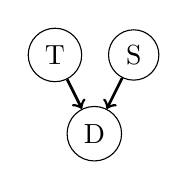
\begin{tikzpicture}
        \node[shape=circle,draw=black] (D) at (0,0) {D};
        \node[shape=circle,draw=black] (T) at (-0.5,1) {T};
        \node[shape=circle,draw=black] (S) at (0.5,1) {S};
        \path [->,line width=1pt] (T) edge node[left]{}(D);
        \path [->,line width=1pt] (S) edge node[left]{}(D);
    \end{tikzpicture}

    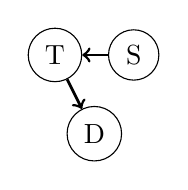
\begin{tikzpicture}
        \node[shape=circle,draw=black] (D) at (0,0) {D};
        \node[shape=circle,draw=black] (T) at (-0.5,1) {T};
        \node[shape=circle,draw=black] (S) at (0.5,1) {S};
        \path [->,line width=1pt] (S) edge node[left]{}(T);
        \path [->,line width=1pt] (T) edge node[left]{}(D);
    \end{tikzpicture}
    \end{center}  
\end{multicols}

\begin{enumerate}[label=(\alph*)]
    \item How many independent parameter values are required to fully define each distribution?
    \item Suppose you are an app developer who wants to warn users how likely it is that they will be delayed based on the temperature and snow history. Your data scientist fits a model in the form on the right because ``it has fewer parameters so it is better'' and gives it to you. How do you respond?
\end{enumerate}

\end{question}

\begin{samepage}
\begin{question}
    Consider the Bayes Net below:
\begin{center}
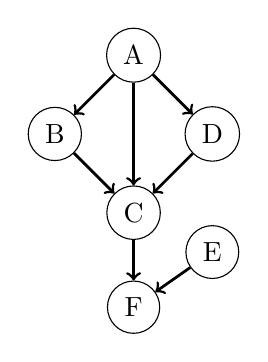
\begin{tikzpicture}
    \node[shape=circle,draw=black] (A) at (0,0) {A};
    \node[shape=circle,draw=black] (C) at (0,-2) {C};
    \node[shape=circle,draw=black] (B) at (-1,-1) {B};
    \node[shape=circle,draw=black] (D) at (1,-1) {D};
    \node[shape=circle,draw=black] (E) at (1,-2.5) {E};
    \node[shape=circle,draw=black] (F) at (0,-3.2) {F};
    \path [->,line width=1pt] (A) edge node[left]{}(B);
    \path [->,line width=1pt] (A) edge node[left]{}(C);
    \path [->,line width=1pt] (A) edge node[left]{}(D);
    \path [->,line width=1pt] (B) edge node[left]{}(C);
    \path [->,line width=1pt] (C) edge node[left]{}(F);
    \path [->,line width=1pt] (D) edge node[left]{}(C);
    \path [->,line width=1pt] (E) edge node[left]{}(F);
\end{tikzpicture}
\end{center}

\begin{enumerate}[label=(\alph*)]
    \item Suppose that you want to know the value of $D$ with the highest precision possible. Allie knows the value of $A$, Brian knows the value of $B$. You can only talk to one of these people. Who should you ask?\footnote{Hint: Consider potential conditional independence relationships such as $(A \perp D \mid B)$.}
    \item Suppose that you already know the values of $F$ and $A$ and want to guess the value of $D$. Eric knows the value of $E$ and Brian knows the value of $B$. You can only talk to one of these people. Who should you ask?
\end{enumerate}
\end{question}
\end{samepage}

\section{Exercises}

\begin{question}
    Consider two stochastic processes, $\{x_t\}$ and $\{y_t\}$, defined by $x_t = f_x(x_{0}, x_{1}... , x_{t-1}, v_t)$ and $y_t = f_y(y_{0}, y_{1}... , y_{t-1}, v_t)$ where $v_t$ are independent, identically distributed random variables that introduce noise. The \texttt{HW1} module in \texttt{DMUStudent} contains two Julia functions, \texttt{fx} and \texttt{fy}, which can sample from the stochastic processes, i.e. \texttt{fx([x1, x2])} will return a sample of $x_3$ given that $x_1 = \texttt{x1}$ and $x_2 = \texttt{x2}$.

    Suppose you know that one of these processes is Markov and the other is not. By drawing samples with the Julia functions, determine which one is Markov.
\end{question}

% \begin{question}
%     A dataset of Titanic passengers is contained in the 
% \end{question}


\section{Challenge Problem}

\begin{question}
    Write a function in Julia that takes in two arguments and uses the Pythagorean Theorem to compute the hypotenuse of a right triangle with side lengths specified by the arguments. Submit this function with \texttt{DMUStudent.submit}. A score of 1 will receive full credit.\footnote{This particular "Challenge Problem" is not meant to be challenging; it is meant to test that everyone can download the code and submit. It should require only 2 lines. Future problems in this section will be quite challenging.}
\end{question}

\end{document}
